\documentclass[11pt]{article}

%####### DON'T CHANGE MARGIN SETTINGS ###########
\newcommand{\keywordfont}{\textsc}
\newcommand{\keyword}[1]{%
  \marginpar{\raggedright\small\keywordfont{#1}}}
\reversemarginpar
\usepackage[a4paper, top=2.5cm, bottom=2.5cm, outer=2cm, inner=3.3cm, marginparwidth=72pt, heightrounded]{geometry}
%#################################

\usepackage{amsmath}
\usepackage{amssymb}
\usepackage{hyperref}
\usepackage{graphicx}
\usepackage{microtype}
\usepackage{mathtools}

\begin{document}

\Large
\begin{center}
\textbf{MA3K7 Week $8/9$ Rubric}
\\
Timothy Yap (2161367)
\end{center}
\normalsize



%-----------------------------------------------------------------------------------------------------------

% You are standing on the first step of an infinitely long numbered path. | 1 | 2 | 3 | 4 | ...

% You have a fair coin which has the number 1 written on one side and the number 2 on the other. You throw the coin, and if it comes up N, you would then take N steps to the right. 
% For example, if you throw the coin and it comes up 2, you take 2 steps to the right to land on step number 3.
% You now repeat the exercise, throwing the coin again and walking the number of steps that comes up on the coin. If you throw the coin 24 times, you are certain to have landed on, or past, step number 25. 

% What is the probability that at some point in this exercise you will land on step number 25? 

\section{Entry} %-------------------------------------------------------------------------------------------



We have a fair coin \keyword{I know} that gives us a 50\% chance of moving one step or a 50\% chance of moving two step along our numbered path. 

We take \keyword{Introduce} \textit{$i$ steps} depending on the value obtained through our coin flip. To reduce confusion between $i$ steps and step numbered $k$, we will say \textit{position $k$} on our numbered path. We also consider a \textit{turn} to be a flip of our coin and the value obtained from it.

\keyword{I know}
\begin{itemize}
    \item We will land on or past 25 after 24 turns.  
    \item There are only two ways of landing on 25 in one turn; either start our turn on 24 and flip a 1 or start at 23 and flip a 2. 
\end{itemize}

\keyword{I want}
\begin{itemize}
    \item  What is the probability of landing on position 25 during the exercise. 
    \item What are the different possibilities of reaching position 25.
\end{itemize}

Before trying to \keyword{Assumptions} answer the question, we assume that once we step on or past 25, the further steps don't impact our chances. Thus, despite being on an infinitely long path, all later turns beyond this won't affect our probability.

Finally, \keyword{Introduce} we introduce the following notation: $a \xrightarrow[]{+i} b $ where $b$ is our ending position after adding $i$ steps to our starting position $a$. For now $i \in \{1, 
2\}$. This can be used iteratively, e.g. $a \xrightarrow[]{+i_1} b \xrightarrow[]{+i_2} c$. We will use $x$ to denote this final position.



%-----------------------------------------------------------------------------------------------------------

\section{Attack} %------------------------------------------------------------------------------------------



We begin \keyword{Strategic Specialisation} by reducing our problem to reaching smaller values, say $x$. Starting on step 1, to get to position $x=2$, we have one turn to flip a 1. This gives us a 50/50 chance. Moving to $x=3$, we could go straight from position 1 to 3 by moving 1 step twice or 2 steps once. Similarly for $x=4$ and $x=5$, we show this as below using the above notation.

\[
x=2 \implies 1 \xrightarrow[]{+1} 2 
\]
\[
x=3 \implies 1 \xrightarrow[]{+1} 2 \xrightarrow[]{+1} 3, \text{    or     } 1 \xrightarrow[]{+2} 3  
\]
\[
x=4 \implies 1 \xrightarrow[]{+1} 2 \xrightarrow[]{+1} 3 \xrightarrow[]{+1} 4, \text{   or    } 1 \xrightarrow[]{+1} 2 \xrightarrow[]{+2} 4, \text{   or    } 1 \xrightarrow[]{+2} 3 \xrightarrow[]{+1} 4
\]
\[
x=5 \implies 1 \xrightarrow[]{+1} 2 \xrightarrow[]{+1} 3 \xrightarrow[]{+1} 4 \xrightarrow[]{+1} 5, \text{   or    } 1 \xrightarrow[]{+1} 2 \xrightarrow[]{+1} 3 \xrightarrow[]{+2} 5, \text{   or    } 
\]
\[
1 \xrightarrow[]{+1} 2 \xrightarrow[]{+2} 4 \xrightarrow[]{+1} 5, \text{   or    } 1 \xrightarrow[]{+2} 3 \xrightarrow[]{+1} 4 \xrightarrow[]{+1} 5, \text{   or    } 1 \xrightarrow[]{+2} 3 \xrightarrow[]{+2} 5
\]


Firstly, we note \keyword{AHA} that we get more permutations the larger our $x$ is. Thus, this method of writing all possible permutations out isn't feasible  for larger values of $x$. Next, we always get the possible combination of always moving 1 step up to $x$. If $x-1 \equiv 0 \text{ mod } 2$, then there is also the possible combination of always moving 2 steps till $x$. Lastly, we can also see that the order doesn't matter. Going 2 steps then 1 steps is the same as going 1 step and then 2 steps.

Attempting to \keyword{Stuck} generalise what we noted above, still seemed exhaustive. We pivot and introduce new notation, a \textit{tuple} $(i_1, i_2, \dots, i_k)$\keyword{Introduce} to describe the path we took. For example, going from position 1 to position 4 we could have the tuples $(1, 1, 1)$, $(1, 2)$ or $(2, 1)$. 
We now instead try \keyword{Try} writing down the probabilities instead.

\begin{table}[h]
    \centering
    \renewcommand{\arraystretch}{1.2}
    \begin{tabular}{|c|c|l|l|} \hline 
         $x$&  Possible Tuples &Explanation &Probability \\ \hline
         2&   (1)&We have to flip a 1 &$\frac{1}{2} = 1 \times \frac{1}{2}$\\ \hline
 3&  (1, 1), or (2)&We either flip 1 twice or 2 once&$\frac{3}{4} = (\frac{1}{2} \times \frac{1}{2}) + \frac{1}{2}$\\ \hline
         4&   (1, 1, 1), (1, 2), or (2, 1)& We can add 2 from position 2 &$\frac{5}{8} = (\frac{1}{2} \times \frac{1}{2}) + (\frac{1}{2} \times \frac{3}{4})$\\
 & & or add 1 from position 3& \\ \hline
 5& (1, 1, 1, 1), (1, 1, 2), & We can add 2 from position 3 & $\frac{11}{16}= (\frac{1}{2} \times \frac{3}{4}) + (\frac{1}{2} \times \frac{5}{8})$\\
 & (1, 2, 1), (2, 1, 1), or (2, 2)& or add 1 from position 4& \\ \hline 
    \end{tabular}
    \caption{Probability Values}
    \label{tab:my_label}
\end{table}

While calculating  \keyword{AHA} the probability, we found a pattern that uses the fact that in order to reach position $x$ either have to start from position $x-1$ and flip a 1 or  start from position $x-2$ and flip a 2. We could have possibly seen this earlier as it is stated in what we know. In either case, we know that we have a $\frac{1}{2}$ chance of flip a 1 or a 2. Thus we \keyword{Conjecture} conjecture the following:
The probability of landing on step $x$ is
\[
p(x) = \frac{1}{2} \times p(x-1) + \frac{1}{2} \times p(x-2)
\]
We let $p(x)$ denote the \keyword{Introduce} probability of landing on position $x$. From Table 1, $p(2) = \frac{1}{2}$ and $p(3)=\frac{3}{4}$. In order \keyword{Justify} to see this works, we know that there are only two possible positions to be in before reaching position $x$, that is $x-1$ and $x-2$, as stated above. We must flip either a 1 or 2 which both have a 50\% probability respectively. That is where the the coefficient of $p(x-1)$ and $p(x-2)$ come from. As we can build our probabilities up from our base case of $x=2$ and $x=3$, then we can calculate any $p(x)$.  
 
We can also try \keyword{Try} using Python to simulate many exercises and using that data to calculate the probability of landing on $x$. In our implementation, we stop our function once it reaches $x$ or $x+1$ and add up all the times we land on $x$ over the number of times we ran our simulation. We get the following data:
\begin{table}[h]
    \centering
    \renewcommand{\arraystretch}{1.3}
    \begin{tabular}{|c|c|c|c|c|c|} \hline 
          $x$&2&  3&  4&  5&  6\\ \hline 
          Simulated Probability&0.49999587&  0.74996177&  0.62491947&  0.68749202&  0.65628453\\ \hline 
 Actual Probability& $\frac{1}{2}=0.5$& $\frac{3}{4}=0.75$& $\frac{5}{8}=0.625$& $\frac{11}{16}=0.6875$&$\frac{21}{32} = 0.65625$\\ \hline
    \end{tabular}
    \caption{Simulated Probability}
    \label{tab:my_label}
\end{table}


With each exercise ran 100 million times, we are confident enough to believe our conjecture. Attempting with  a billion exercises for $x=25$ we obtain a value of 0.666651396. \keyword{AHA}  Calculating with our formula we obtain a value of 0.6666666865348816. From this, we state \keyword{Conjecture} the following conjecture:
\[
\text{As} \hspace{10pt} x \rightarrow \infty \hspace{10pt} \text{then} \hspace{10pt} p(x) \rightarrow \frac{2}{3}
\]
Using Python code from Lab 7, \keyword{Justify} we find that the explicit formula for our first conjecture is $\frac{1}{3}(-0.5)^{x-1}+\frac{2}{3}$ so we can see that as $x \rightarrow \infty$ our first term will tend to 0, leaving $\frac{2}{3}$ as the remaining term. Thus proving our conjecture. 

\begin{figure}[h]
   \centering
   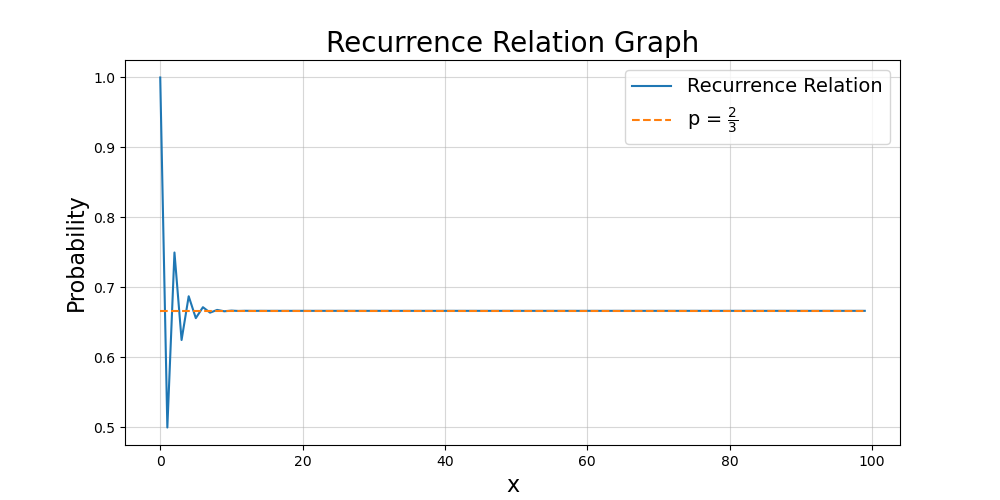
\includegraphics[width=5.5in]{RRgraph.png}
   \label{myfig}
\end{figure}

Again, we \keyword{Check} turn to Python to plot the above graph. We can see that the our recursive function tends to the desired $\frac{2}{3}$. We plot our function up to $x=100$ to show that for even larger values of $x$, our conjecture holds. From the graph, we can see that even with $x=10$, the graph is already near $\frac{2}{3}$. Putting $x=10$ into our explicit formula, we get $\frac{1}{3}(-0.5)^{10-1}+\frac{2}{3} = 0.666015625$ which is already an absolute difference of 0.0006510\dots .\\


Moving on to find the number of different possibilities of landing on 25, we begin with some of our initial observations. We have a tuple (1, 1, \dots, 1) of size 24. If we pair two 1's, say the first pair, we get an new tuple (2, 1, 1, \dots, 1) of size 23. We now move this pair to the right and obtain (1, 2, 1, \dots, 1). However, this method gets much more complicated when we introduce multiple 2's as we have to account for various combinations. Instead we notice that the possible tuples follow a pattern of 1, 2, 3, 5, \dots which relate to the Fibonacci sequence. So working with this, we find that 1, 2, 3, \dots, 28657, 46368, 75025 is our sequence up to $x=25$. There are 75025 different possibilities of reaching 25.

%-----------------------------------------------------------------------------------------------------------

\section{Review} %------------------------------------------------------------------------------------------

Returning \keyword{Check} to our initial questions, we found the answer to what is the probability of landing on 25 to be 0.666666686534881, which is an approximation of the actual answer of $\frac{11184811}{16777216}$. Something to note is that 16777216 is $2^{24}$ which comes from that fact that each iteration halves the previous two iteration. We also found that there are 75025 different ways of getting to 25, and that the number of permutations follows the Fibonacci sequence. 

I initially thought \keyword{Reflect} the answer was as simple as a $\frac{1}{2}$ as you either flip a 1 and step on 25 or flip a 2 and pass 25. Quite obviously, you could land on 23 and flip 2, landing on 25. Another lapse of judgement was when I thought the answer might be $(\frac{1}{2})^{24}$ as I assumed, incorrectly, one must roll 24 times. Thus the only way is to roll 24 ones. Luckily, these were very early mistakes that made me read the question extra carefully. 

Anther setbacks \keyword{Reflect} that I encountered was trying to calculate the probability of each $x$. Despite my initial setback, it ended up still being useful to have as that is how I found that the number of possible paths follows the Fibonacci sequence. Writing in a table format gives a better perspective which is also how I figured out the recursive formula. This should have been quite obvious from the fact that I stated the only way to reach 25 was from 24 or 23 and flipping a 1 or 2 respectively. However, listing it down did help me have it in the back of my mind when calculating probabilities. 
 
Throughout \keyword{Reflect} this essay, Python was used to calculate various equations. I had quite quickly implemented a function to find whether a path was successful in landing on 25. With that, I was able to simulate the exercise a billion times to find it averaged around the above. However, with this alone, I didn't have enough information to conclude that the limit was $\frac{2}{3}$. Working from the ground up with the help of Python was necessary. In order to test a large number of exercises, I tested different functions for efficiency. In my code, I tested the two functions below to see which was better at generating random steps.
\begin{verbatim}
1 + random.getrandbits(1)
np.random.randint(1, 3)
\end{verbatim}
At first, I used the second function but found that the first function had generated random step sizes much faster. Testing between the two found that the first function was 20 to 30 times faster. This is especially helpful when simulating a billion exercises. Despite this, even using the second function and 10 million exercises would have been enough. Lastly, Python code was used from Lab 7 to generate an explicit formula which helped explain why for larger $x$, probability converges to $\frac{2}{3}$.
  
Changing our \keyword{Extend} initial question, there are a number of different extensions we could have.

\begin{itemize}
    \item Different ways of obtaining N :
    \begin{itemize}
        \item Have a dice instead of a coin so we have a greater number of choices for step size.
        \item Have step sizes of different values; e.g. 2 and 3.
        \item Have negative steps: e.g. -1 and 2.
        \item Change the likelihood of obtaining a certain value.
        \item         A combination of the above: e.g. a six-sided die with faces 1, 4, 7, -1, -2, -3 and respective probabilities of 10\%, 10\%, 20\%, 20\%, 20\%, and 20\%.
    \end{itemize}
    \item Start and end at a different value (or multiple values).
    \item Only flip our coin $y$ times. For our set up we would need $y < 24$.
    \begin{itemize}
        \item We could have a finite path; where at the end we step backwards which would allow for $x$ to be bigger than 24 but still give us a possibility to not land on 25.
    \end{itemize}
\end{itemize}

We try two of our \keyword{Extend} extensions, 1) adding a fair four-sided die, and 2) starting and ending at different values.

For our first extension, \keyword{Extend} we have a 25\% chance of stepping 1, 2, 3, or 4 steps. We use a similar idea that to reach 25, we can either start from position 21, 22, 23, or 24 and move 4, 3, 2, or 1 step(s) respectively. Starting on pose need our 'base' probabilities as shown in the following table:

\begin{table}[h]
    \centering
    \begin{tabular}{cccc}
         $x$&  Possible Tuples&  Calculations& Probability\\
         2&  (1)&  $= 1 \times \frac{1}{4}$& $\frac{1}{4}$\\
         3&  (1, 1), or (2)&  $=  \frac{1}{4} \times \frac{1}{4} + \frac{1}{4}$& $\frac{5}{16}$\\
         4&  (1, 1, 1), (1, 2), (2, 1), or (3)&  $=  \frac{1}{4}^3 + 2 \times \frac{1}{4}^2 + \frac{1}{4}$& $\frac{25}{64}$\\
         5&  (1, 1, 1, 1), (1, 1, 2), (1, 2, 1),&  $=  \frac{1}{4}^4 + 3 \times \frac{1}{4}^3 + 3 \times \frac{1}{4}^3 + \frac{1}{4}$& $\frac{125}{256}$\\
 &  (2, 1, 1), (2, 2), (1, 3), (3, 1), or (4)& &\\
    \end{tabular}
    \caption{Probability Values for Extension}
    \label{tab:my_label}
\end{table}
We see that the binomial expansion when $x=5$ which relates to the aforementioned Fibonacci sequence (as the sums of the diagonals of Pascal's Triangle) \keyword{I know}. We also see that the probability follows the following form: $\frac{5^{x-2}}{4^{x-1}}$. Obviously, this does not follow for the greater values of $x$ as for large $x$, $p(x) > 1$ which is impossible. With our base case, we have the following recursive formula:
\[
p(x) = \frac{1}{4} \times p(x-1) + \frac{1}{4} \times p(x-2) + \frac{1}{4} \times p(x-3) + \frac{1}{4} \times p(x-4)
\]

Implementing this into \keyword{Try} Python we find that our value for $x =25$ is 0.39999238267585113. We also plot the graph below to show that our parameters converge to $\frac{2}{5}$. Again at $x=10$ the relation converges quite fast.

\begin{figure}[h]
   \centering
   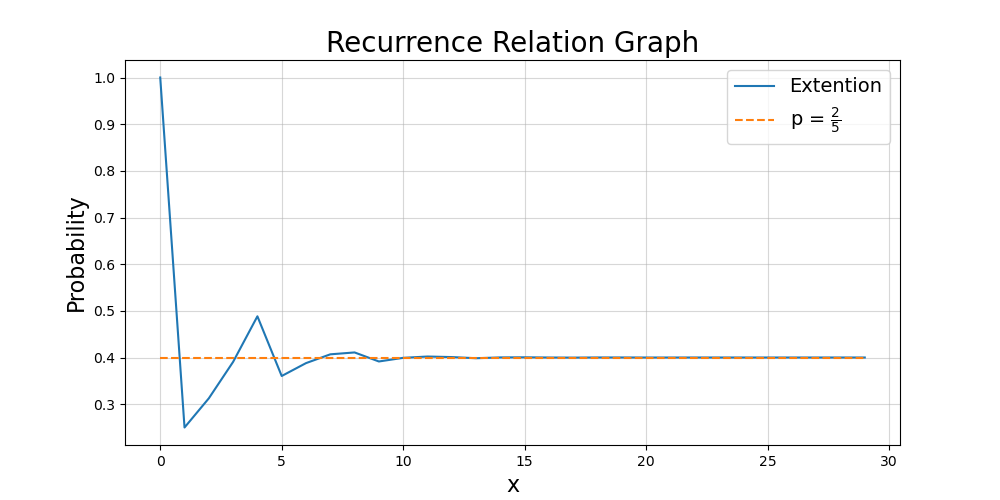
\includegraphics[width=5.5in]{ExtGraph.png}
   \label{myfig}
\end{figure}



Moving onto our second extension, \keyword{Extend} we start at 25 and end at $x=50$. Again, we build on what we have already gone through. Now instead of having a 50\% chance of landing on position 2 from position 1, we have a 50\% chance of landing on position 26 from position 25. However, using Python,  \keyword{Try} we find that the probability stays the same. This is likely due to the fact that the probability of rolling either a 1 or 2 is also the same. Shifting our starting and ending positions has no applicable effect on our probability. Thus, we converge to $\frac{2}{3}$, similar to our starting parameters. 

Overall, \keyword{Reflect} this has been an enjoyable exploration of our given problem. With more effort, we could find how all the different starting parameters may affect the probability, but currently, we now know that starting positions don't matter but the probability of our steps does. With further expansion, we could investigate how different step sizes affect the convergent probability. Just intuitively, larger steps would make convergence happen later, or more precisely, for comparatively larger values of $x$.

\section*{Supplementary material}
The code for this assignment can be found on my GitHub page:  \url{https://github.com/LazyTim/MA3K7/blob/main/MA3K7%20-%20Assignment%204.ipynb}.

\end{document}
